\section{error control instead of defect control}
Another idea is to consider error control instead of defect control for the continuous approximate solution. We would thus need a way to create two interpolants, one of a higher order and one of a lower order and sample the difference between these two interpolants to estimate the error of the continuous solution approximation. 
=== A step-size selection algorithm based on that error estimate could provide an effective error controlled solution.

An issue with defect control is the V-shape of the defect. 
We know that this is entirely because of the $\frac{1}{h}$ in the derivative definition of the Hermite-Birkhoff interpolants as the interpolant itself does not suffer from round-off error but its derivative does.

\subsection{error is not v-shaped}
For all the schemes, the defect is V-shaped but the error itself is not. 
This is because the Hermite-Birkhoff interpolant does not contain a term in $\frac{1}{h}$ whereas its derivative does contain such a term. 
Figure $\ref{fig:defect_is_v_shape}$ and $\ref{fig:error_is_not_v_shape}$ shows this phenomenon for HB6 but the same can be see for HB4 and HB8. 

\begin{figure}[H]
\centering
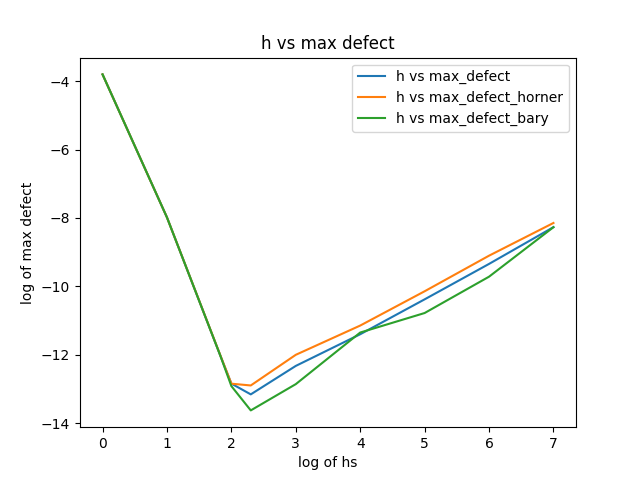
\includegraphics[width=0.7\linewidth]{./figures/further_work_defect_is_v_shape_hb6}
\caption{Defect has V-shape.}
\label{fig:defect_is_v_shape}
\end{figure}

\begin{figure}[H]
\centering
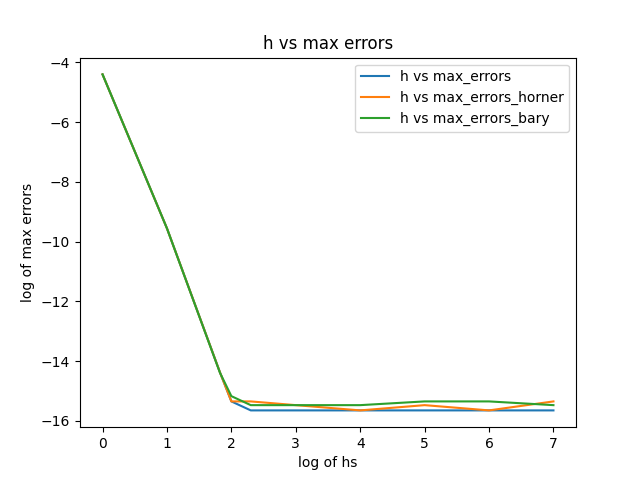
\includegraphics[width=0.7\linewidth]{./figures/further_work_error_is_not_v_shape_hb6}
\caption{Error does not have V-shape.}
\label{fig:error_is_not_v_shape}
\end{figure}

\subsection{sampling error}
we sample
\begin{equation}
| h(x) - l(x) |
\end{equation}
at two x values within $x_i$ and $x_{i+1}$ and take the max to get the error estimate within the step.

\subsubsection{rk4 with hb4 vs hb6}
Because we do not differentiate and that hb4 has order 4, we can use with rk4 with HB4 for error control. Thus HB4 and HB6 should not suffer from much interpolation error and we can use rk4 with the hb4 and hb6 using the error scheme

\subsubsection{rk4 with hb6 vs hb8}
rk4 can also be use with hb6  and hb8 and not suffer from much interpolation error.

\subsubsection{rk6 with hb6 vs hb8}
Because we do not differentiate and that hb6 has order 6, we can use with rk6 with HB6 for error control. Thus HB6 and HB8 should not suffer from much interpolation error and we can use rk6 with the hb4 and hb6 using the error scheme

\subsubsection{continuous L2 norm}
The error estimate is calculated with a continuous L2 norm as follows.
\begin{equation}
error_i = \sqrt{ \int_{x_i}^{x_{i+1}} (\frac{h(x) - l(x)}{1 + |l(x)|})^2 \,dx }
\end{equation}
where h(x) is the higher order interpolant and l(x) is the lower order interpolant. This formula gives the error for one step and we compare it with the user provided atol for error control. 

========================
We ignored rtol as we had to factorise tol from the denominator so that we can use tol and $tol/10$ for comparisons. Essentially we assume $atol == rtol$
===================

\subsubsection{rk4 with hb4 vs hb6}
Because we do not differentiate and that hb4 has order 4, we can use with rk4 with HB4 for error control. Thus HB4 and HB6 should not suffer from much interpolation error and we can use rk4 with the hb4 and hb6 using the error scheme

\subsubsection{rk4 with hb6 vs hb8}
rk4 can also be use with hb6  and hb8 and not suffer from much interpolation error.

\subsubsection{rk6 with hb6 vs hb8}
Because we do not differentiate and that hb6 has order 6, we can use with rk6 with HB6 for error control. Thus HB6 and HB8 should not suffer from much interpolation error and we can use rk6 with the hb4 and hb6 using the error scheme

\subsection{conclusion}